The workflow of the underwriting, buying, and settlement process, as well as the claim procedure, is depicted in the two charts below.
Here are the main parts of the system.

\begin{figure}[H]
	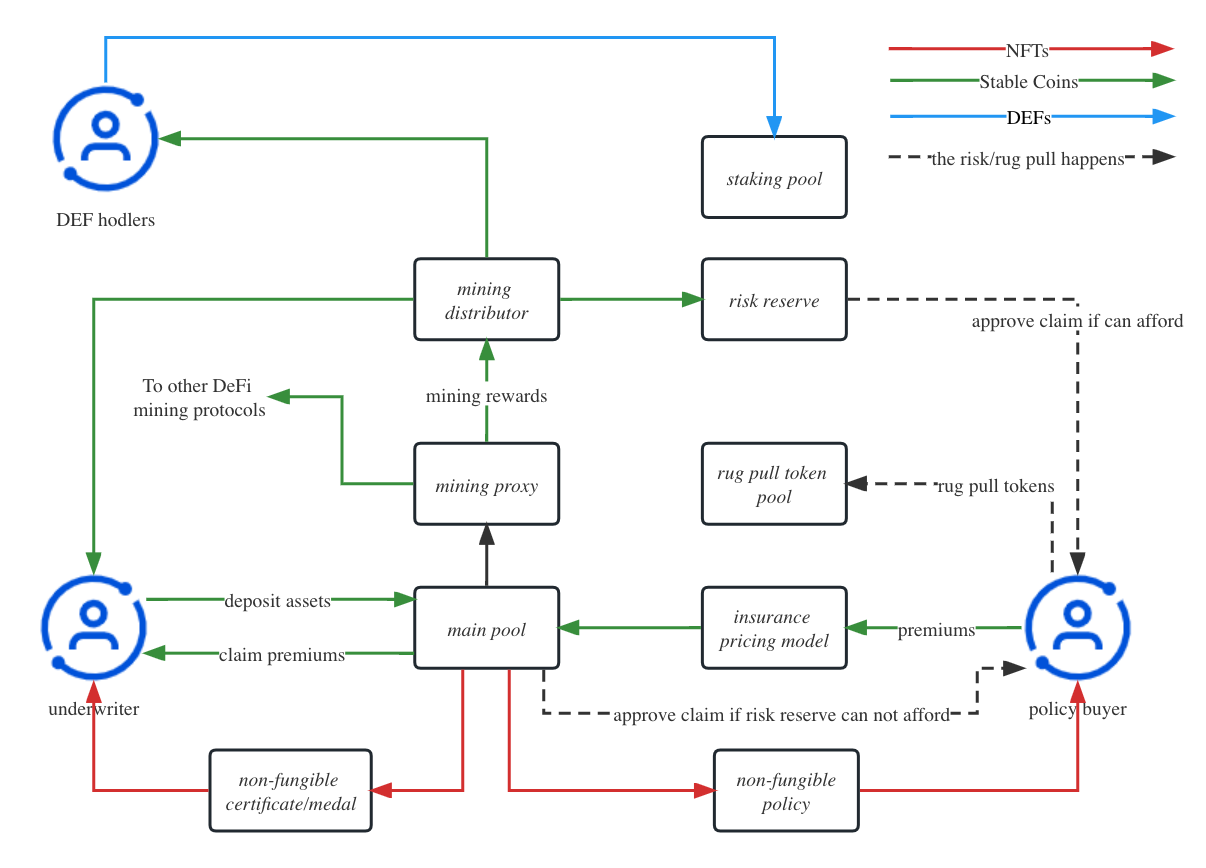
\includegraphics[width=\linewidth]{../workflow_process_on} % Figure image
	\caption{MetaDefender Workflow} % Figure caption
	\label{fig:workflow} % Label for referencing with \ref{bear}
\end{figure}

\begin{itemize}
    \item main pool: The key component of the system.
	The (total value locked)TVL in the pool is made up of three components: the underwriters' assets given, the premium paid by policyholders, and the unfrozen assets temporarily held for some underwriters' early departures.
	\item insurance pricing model: The premium computation portion.
	It employs the American binary option formula to estimate the insurance premium using the policy duration and policy coverage as input parameters.
	\item non-fungible certificate/policy: The NFT is responsible for the liquidity certificate and policy.
	The NFT is coined and transmitted to the user when the user underwrites/purchases insurance.
	The NFT adheres to the ERC721 standard, and users can sell their liquidity at any moment.
	\item risk reserve: Because preserving underwriters' capital SAFU is vital, a portion of the mining rewards will be transferred to the risk reserve pool.
	If the risk situation occurs and policyholders apply for claims, the protocol will initially use the funds in the risk reserve pool rather than the main pool.
	If the funds are inadequate to cover all claims, the main pool will step in to pay the rest of money, putting the underwriters' capital at risk.
	\item DAO: The DAO is made up of numerous stakeholder groups, including the MetaDefender team, insurance specialists, the EVM safety team, and DEF hodlers.
	They vote in the DAO voting system to determine if we will approve the claim after a thorough investigation of the issue.
\end{itemize}
